\ifdefined\PROCINCLUDED
%
\else
%%% Please, do not change any of the following parameters.
\documentclass[b5paper,twoside,11pt]{article}
\usepackage[utf8]{inputenc}
\usepackage{geometry}
\voffset=-0.04cm
\headheight=0.6cm
\headsep=0.65cm
\textheight=19.5cm
\footskip=1.25cm
\voffset=-0.04cm
\textwidth=12.6cm
\marginparsep=0cm
\oddsidemargin=0cm
\evensidemargin=0cm
\marginparwidth=0cm
\usepackage{fancyhdr}
\usepackage{url}
\usepackage{graphicx}
\usepackage{mathptmx}
\usepackage{amsmath}
\usepackage{float}
\usepackage{subcaption}
\usepackage{placeins}
\usepackage{gensymb}
\usepackage[labelsep=period]{caption}
\captionsetup[table]{skip=7pt}
\captionsetup[figure]{skip=6pt}
\fancyhead{}
\fancyfoot{}
\fancyfoot[LE]{\thepage}
\fancyfoot[RO]{\thepage}
\renewcommand{\headrulewidth}{0.4pt}
\renewcommand{\footrulewidth}{0pt}
\date{}
\def \papertitle#1{\title{#1}}
\pagestyle{fancy}
\def\insertauthor#1#2{
	\begin{minipage}[t]{.45\textwidth}
		\centering
		{\em#1} \\ \vspace*{0.25em}
		#2 \\ \vspace*{1.25em}
	\end{minipage}
}
\def\paperauthors#1{
	\author{
	\begin{minipage}[t]{\textwidth}
	\centering
	#1
	\end{minipage}
	}
}
\def\email#1{\\{\small\protect\url{#1}}}
\def\runningtitle#1{\fancyhead[CO]{\textit{#1}}}
\def\runningauthor#1{\fancyhead[CE]{\textit{#1}}}
\graphicspath{ {figures/} } %%% put all images file into "figures/" subdirectory

\begin{document}
\fi

\papertitle{Contribution title}
\paperauthors{
%%% insert one \insertauthor for each article author, \email part is optional
\insertauthor{Filip Rynkiewicz}{Lodz University of Technology \\ {\L}{\'o}d{\'z}, Poland\email{173186@edu.p.lodz.pl}}
\insertauthor{Stanis{\l}aw Nowak}{MacGilll University \\ Montreal, Canada}
}
\runningtitle{Contribution\dots} %%% brief title for running head
\runningauthor{Kowalski, J. et al.} %%% brief authors for running head


\graphicspath{ {images/} }


\maketitle




\begin{abstract}
Since the beginning of computer era we are trying to imitate nature. The results of those attempts are mathematical equations describing weather, snow flakes, plant growth or influence of species in individual biomes. In computer graphics fractal structure are often used because they can be simple characterize in mathematics. Those forms are common in naure and can be found in example in broccoli, corals, lightnings or in trees. 
Self-similar fractals can be created in computer graphics using Lindermayer Systems. This article was created to analyze efficiency of this algorithm in modeling 3D tree triangle meshes for games. The general motivation of this topic is to produce way to procedural modeling and simplified edition of complicated 3D tree models. By combining L-systems with Bezier Curve there is a possibility to produce complicated 3D models. For example tree created with 468 branches having 87200 vertices and it is made in few seconds. In conclusion, time-consuming modeling in 3D programs can be replaced by solution described in this article. 
\end{abstract}

%%% insert your contribution here

\section{Introduction}
From beginning of our era we are trying to imitate nature. Results of this attempts are descriptions of natural phenomenon using mathematical equations. Those mathematical statements are used for example in weather forecast, simulation of plant growth, creating snowflakes or lightnings. In computer graphics fractal based structure adopted from nature are often used because they can be simply stored as mathematical formula. One of those formulas is \textit{Lindenmayer System}. It allows user to create a mathematical description of appearance, behavior or grow of plant. 
\par Using 3D modeling programs, such as \textit{3ds Max} or \textit{Blender}, to create a complex 3D model of tree is very time consuming, because every branch has to be shaped separately. To speed up and  automatize this process L-system can be used. This article is description of implementation and usage of L-System in Unity3D Game Engine. Problem with procedural generated structures using L-System in it's basic description it's that all algorithms are generating static models. It's mean that user can't move, add or do anything with model without recalculating it all over again. The basic idea to add this feature is to use \textit{Bezier Curve}, and generate the mesh based on it.
 
\subsection{Fractal}
One of the most important feature of fractal is self-similarity. It's mean that every part of fractal is similar to whole fractal and can be calculated by iterating over simple formula, which describe this fractal. Never ending patter is created by scaling fractal. Observation of plants brought some conclusion which shows that every plant can be treat as a very complex fractal, with multiple elements so it can be simplified using \textit{Lindenmayer System}.

\subsection{Lindenmayer System}
L-system was created in 1968 by Hungarian theoretical biologist and botanist from University of Utrecht Artist Lindenmayer. System was originally devised to describe formal description of simple multicellular organisms. With fast development of computer graphics the L-system is used by the modern artist to create plant models and to simulate its growth. The system in based on rewriting rules, like productions. All system are based on string comprasion, evaluation and conversion.
\subsection*{DOL System}
Deterministic and contex free L-system is one of the L-system, where context of the letter have no affect on algorithm. Simple example. When axiom, starting word, is \textit{b} and rules are: $b \rightarrow a$ and $a \rightarrow ab$ with 5 iterations, the example creation is shown at \figurename\ref{DOL}.

\begin{figure}[!htp]
\centering
  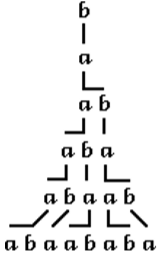
\includegraphics[width=0.2\linewidth]{DOL-system}
\caption{Example of DOL system\cite{prusinABOP} \label{DOL}}
\end{figure}
\subsection*{Bracket L-System}
\section{Methods}

\section{Results}
\subsection*{Example 1}
Rules: \newline
\begin{equation*}
F(l)\rightarrow F(l\cdot2) 
\end{equation*}
\begin{equation*}
X(l) \rightarrow F(l)[/(r)X(l)]F(l)[\setminus(r)X(l)-(r)X(l)]F(l)[\setminus(r)X(l)+(r)X(l)] 
\end{equation*}
Axiom:
\begin{center}
X(1)
\end{center}
Number of iterations:
\begin{center}
5
\end{center}
Variables:
\begin{equation*}
r\rightarrow 25
\end{equation*}
\subsection*{Example 2}
Rules: \newline
\begin{equation*}
F(l)\rightarrow F(l\cdot2) 
\end{equation*}
\begin{equation*}
X(l,w) \rightarrow F(w\cdot l)[/(r\cdot l)X(l,w)-(r)X(w,w)]+(r)F(l)[\setminus(l)X(l,w)+(r)X(l,w)]-(r)F(w)
\end{equation*}
Axiom:
\begin{center}
X(1)
\end{center}
Number of iterations:
\begin{center}
5
\end{center}
Variables:
\begin{equation*}
r\rightarrow 17.2
\end{equation*}

%\item [] $\rightarrow$ 
%\end{itemize}



\subsection*{Example 3}
Rules: \newline
\begin{equation*}
F(l)\rightarrow F(l\cdot2) 
\end{equation*}
\begin{multline*}
X(l,w) \rightarrow F(w\cdot l)[/(r\cdot l)X(l,w)-(r)X(w,w)C(l)]\\
+(r)F(l)[G(l)\setminus(l)X(l,w)+(r)X(l,w)]-(r)F(w)-(r)F(w)
\end{multline*}
\begin{equation*}
G(l) \rightarrow F(l/5)[X(l,l)+(r\cdot k)]
\end{equation*}
\begin{equation*}
C(l) \rightarrow F(l/5)[X(l,l)/(r\cdot k)]
\end{equation*}
Axiom:
\begin{center}
X(1,2)
\end{center}
Number of iterations:
\begin{center}
5
\end{center}
Variables:
\begin{equation*}
r\rightarrow 23.5
\end{equation*}
\begin{equation*}
k\rightarrow 0.707
\end{equation*}





%~~~~~~~~~~~~~~~~~~~~~~~~~~~~~~~~~~
\begin{figure}[!htp]
\centering
\begin{subfigure}{.68\textwidth}
  \centering
  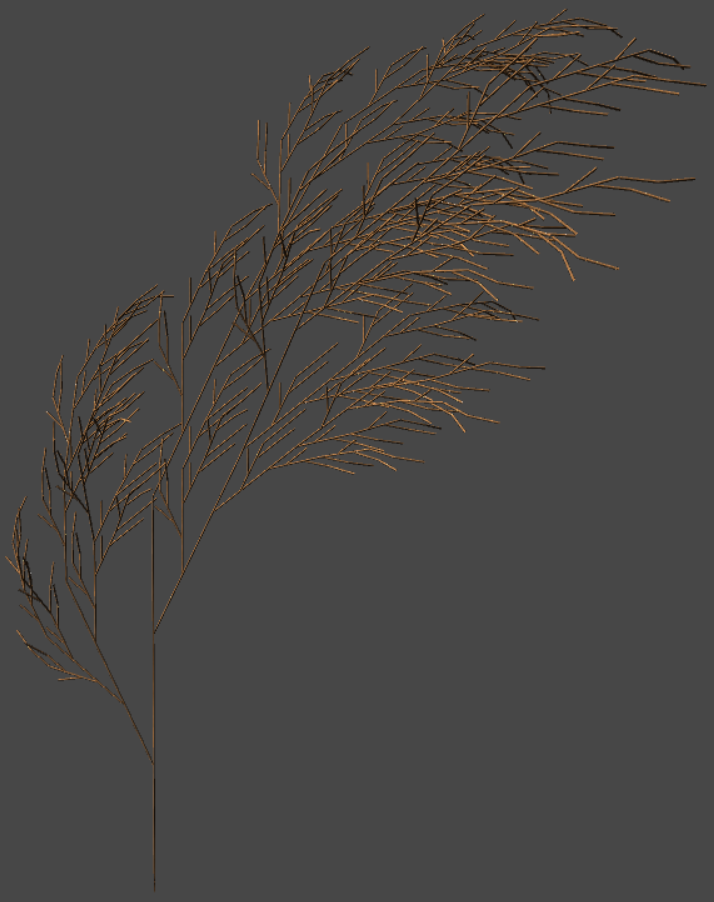
\includegraphics[width=0.8\linewidth]{siatka1}
\caption{Mesh without modification.\\Own source. \label{przyklad1.siatka}}
\end{subfigure}
%
\begin{subfigure}{.68\textwidth}
  \centering
  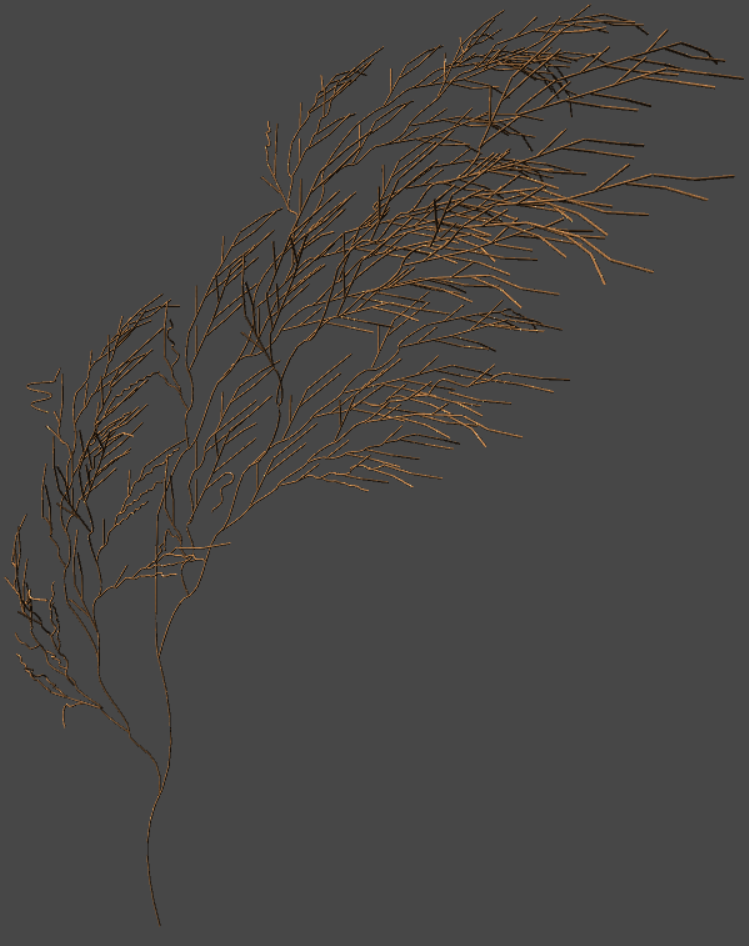
\includegraphics[width=0.8\linewidth]{siatkaMOD1}
\caption{Mesh after modification.\\Own source. \label{przyklad1.siatkaMOD}}
\end{subfigure}
\caption{Comparison of meshes for example  1.}
\label{przyklad1}
\end{figure}
%~~~~~~~~~~~~~~~~~~~~~~~~~~~~~~~~~~
\begin{figure}[!htp]
\centering
\begin{subfigure}{.68\textwidth}
  \centering
  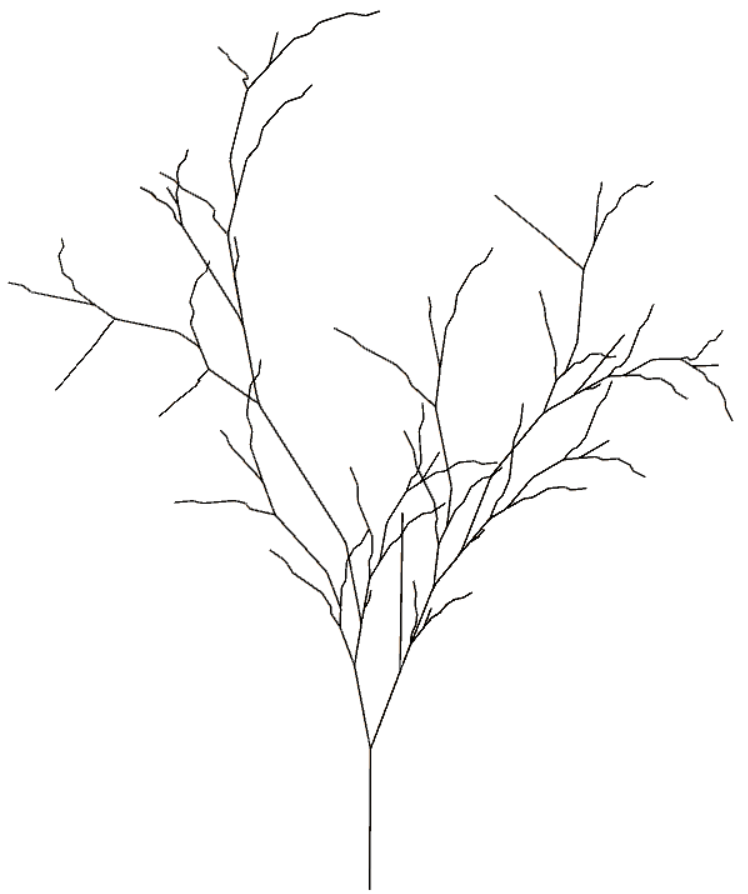
\includegraphics[width=0.8\linewidth]{przyklad2}
\caption{Mesh withouth modification.\\Own source. \label{przyklad2.siatka}}
\end{subfigure}
%
\begin{subfigure}{.68\textwidth}
  \centering
  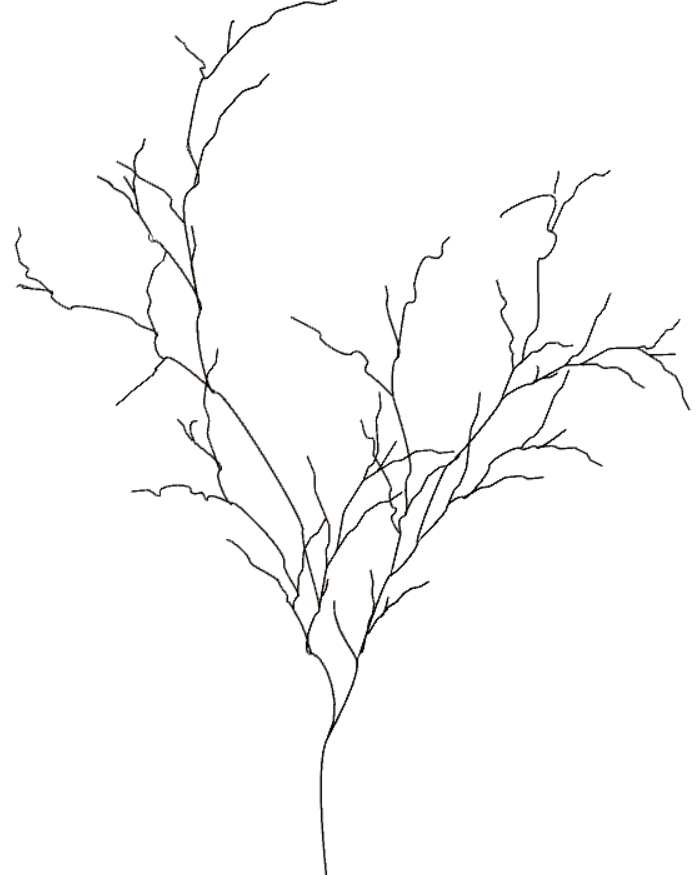
\includegraphics[width=0.8\linewidth]{przyklad2MOD}
\caption{Mesh after modification.\\Own source. \label{przyklad2.siatkaMOD}}
\end{subfigure}
\caption{Comparison of meshes for example  2.}
\label{przyklad2}
\end{figure}
%~~~~~~~~~~~~~~~~~~~~~~~~~~~~~~~~~~
\begin{figure}[!htp]
\centering
\begin{subfigure}{.9\textwidth}
  \centering
  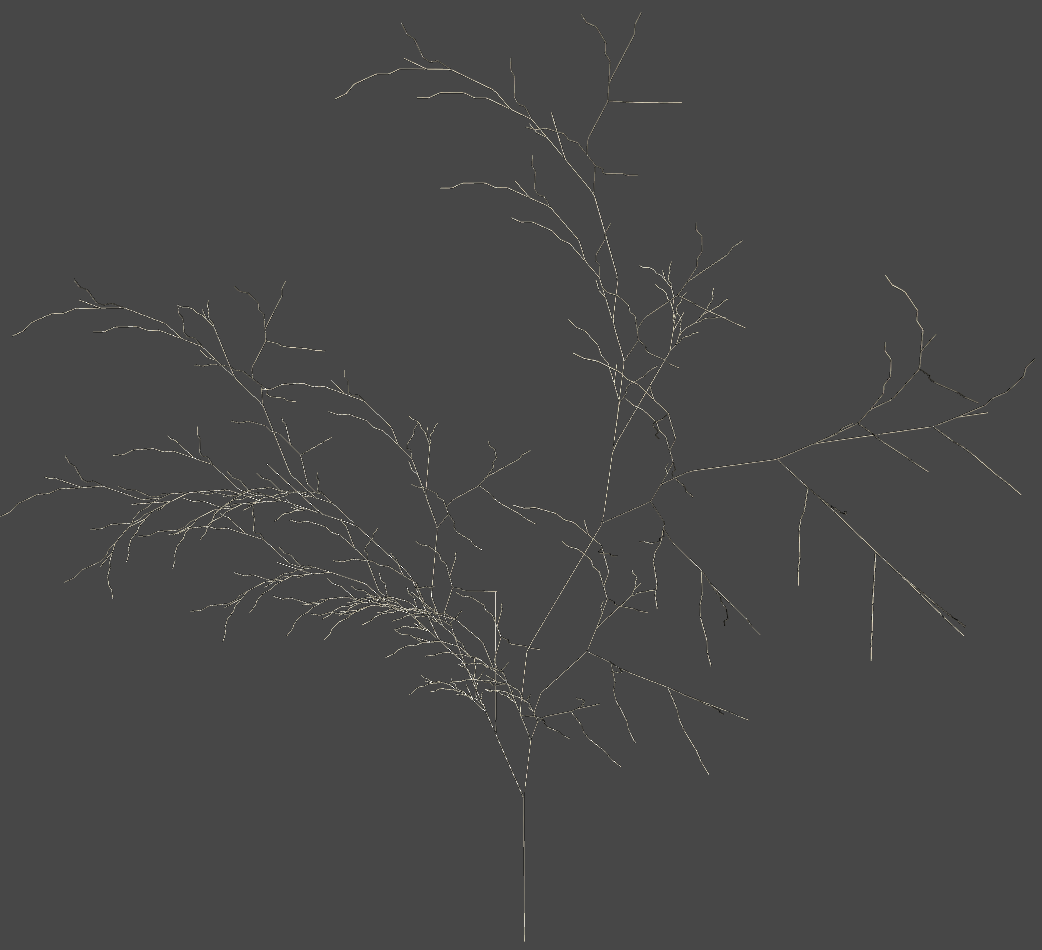
\includegraphics[width=0.8\linewidth]{przyklad3MOD}
\caption{Mesh without modification.\\Own source. \label{przyklad3.siatka}}
\end{subfigure}
%
\begin{subfigure}{.9\textwidth}
  \centering
  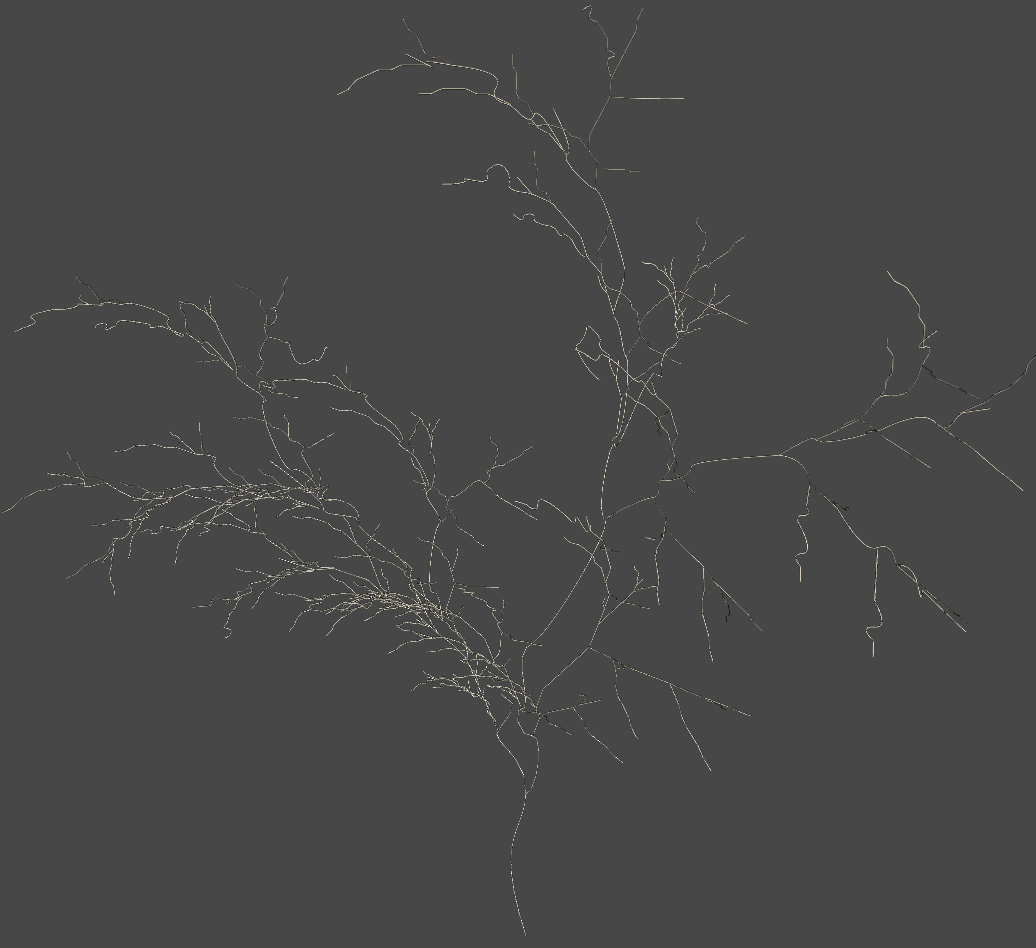
\includegraphics[width=0.8\linewidth]{przyklad3}
\caption{Mesh after modification.\\Own source. \label{przyklad3.siatkaMOD}}
\end{subfigure}
\caption{Comparison of meshes for example  3.}
\label{przyklad3}
\end{figure}
\newpage


\section{Discussion}
For each of the example the same values was used. Five segments on the side surface and five points on spline, it's mean that every curve was divided on five equal parts. Each result of implemented algorithm was divided into two pictures. Screenshot of model generated by algorithm and model after changes. Changes was made by transforming Bezier Points on corresponded to branch Bezier Curve. First all the example and it's description was shown, then the pictures.\par
In first example for 5 iterations the number of branches is 468, word forming tree have 46086 chars and number of vertices in model is 87200.\newline\par
This example is modification of simple fractal plant described in \cite{prusinABOP}.
Every branch is directed at 25  $\degree$ relative to parent branch. As it can be seen at the \figurename \ref{przyklad1.siatka}, the model created by algorithm is complex, using only two rule and one variable. Model after changes have been shown at  \figurename \ref{przyklad1.siatkaMOD}. Every branch in tree have been altered according to user actions.\par 
Next example have 171 branches, world forming tree have 24918 chars and 73700 vertices in model. In this case the custom and longer rules have been used to make model looks like non-deterministic and more chaotic. Model before changes was shown at \figurename\ref{przyklad2.siatka}, and after changes at \figurename\ref{przyklad2.siatkaMOD}. In first example every variable had exactly one parameter without any mathematical operations, except $F(l \cdot 2)$. But in the second example every operation on parameter had to be evaluated and changed to float value, so the time of the calculation had increased significaly. Thanks to usage of multiple parameters and operation between them user can create more complicated structures, using less rules, but for the price of time for parameter evaluations.\par
Last example have 214 branches, world world forming tree have 24918 chars and 73700 vertices in model. POOOOOOOPRAW!!!!!
\figurename \ref{przyklad3.siatka} presents unchanged model of last example, \figurename \ref{przyklad3.siatkaMOD} same model after changes. Creating more complicated rule, based on those in example 2, and adding two more simple rules the model in example 3 is more non-deterministic and tree-like than other examples. Time for creating this tree is not greater than time for example 2, because to store all rules algorith use C\# \textit{Dictionary} where the \textit{Key} is from what chars rule must be changed, and \textit{Value} stores to what rule chars must be changed.


 



\section{Conclusion}
By using technique described before the user can simply generate tree-like model in short time, small amount of vertices, and with ability to change every point of model using Bezier handles. Creating model with 300 branches using normal 3d modeling software would be very time consuming.We can move our work to machine and automatize process of modeling, using simple parameterized mathematical equations, without even knowing how the 3d modeling software works. And we can do this inside game engine, without other programs.

To evaluate all string into float values the simple parser have been created.
Parser created with this implamentation is simple, but creating possibility to evaluate more than 3 parameters, and operations betwen them, using approaches from this implemantation would be very difficult. To ensure that every parameter would be evaluated propertly whole implementation will be rewriten into new \textit{Boost Spirit X3} C++ library, and created as \textit{Dynamic-Link Library}. Unity,Enreal Engine and others game engines have ability to write plugins based on \textit{DLL} written in \textbf{C++}, so every engine could have their own implementation of this algorithm, based on \textit{DLL}.
% use section* for acknowledgement



\begin{thebibliography}{99}
\bibitem{prusinABOP}
Prusinkiewicz P., Lindermayer A. (2004) The Algorithmic Beauty of Plants.  wersja elektroniczna.
\bibitem{wlosy}
Fuhrer M. Hairs, Textures, and Shades: Improving the Realism of Plant Models Generated with L-systems. M.Sc. thesis, University of Calgary, August 2005. wersja elektroniczna
\bibitem{sca}
Runions A., Lane B., Prusinkiewicz P. Modeling Trees with a Space Colonization Algorithm,Department of Computer Science, University of Calgary, Canada ,Eurographics Workshop on Natural Phenomena (2007).
\bibitem{Sub} MacMurchy P., The Use of Subdivision Surfaces in the Modeling of Plants, THE UNIVERSITY OF CALGARY, April, 2004
\bibitem{VertexVertex} Smith C., On Vertex-Vertex Systems and Their Use in Geometric and Biological Modelling, THE UNIVERSITY OF CALGARY, April, 2006
\bibitem{houdiniZrodlo}
http://www.digitaltutors.com/tutorial/570-Procedural-Tree-Growth-Using-L-systems-in-Houdini
\bibitem{speedTreeZrodlo}
\url{http://www.speedtree.com/images/modeler_lrg.jpg}
\bibitem{unity}\url{https://unity3d.com/5}
\bibitem{mono}\url{http://www.mono-project.com/}
\bibitem{splajn}\url{http://www.zobaczycmatematyke.krk.pl/025-Zolkos-Krakow/b-spline.html}
\bibitem{treeSketch}TreeSketch:Interactive Procedural Modeling of Trees on a Tablet, Longay S.,  Runions A., Boudon F., Prusinkiewicz P.
\bibitem{slon}\url{http://kacikzdrowia.pl/wp-content/uploads/2015/01/s%C5%82onecznikb.jpg}
\bibitem{konw}\url{https://sadzawka.pl/Convallaria_majalis_Aurea-Konwalia_majowa}
\bibitem{stringBuilder}\url{https://msdn.microsoft.com/pl-pl/library/system.text.stringbuilder%28v=vs.110%29.aspx}
\bibitem{dict}\url{http://net-informations.com/faq/general/dictionary-list.htm}
\bibitem{bezUnity}\url{https://www.assetstore.unity3d.com/en/#!/content/11278}
\bibitem{youtube}\url{https://www.youtube.com/watch?v=o9RK6O2kOKo}
\bibitem{unityMesh}\url{http://docs.unity3d.com/Manual/class-MeshRenderer.html}
\bibitem{MBN}\url{http://jayelinda.com/modelling-by-numbers-part-1a/}
\bibitem {LMat} Rozenberg G., Salomaa A. \textit{The mathematical theory of L systems}, Academic Press, New York, 1980
\end{thebibliography}

\ifdefined\PROCINCLUDED
%
\else
\end{document}
\fi
